% mnras_guide.tex
%
% MNRAS LaTeX user guide
%
% v3.0 released 22 May 2015
% (version numbers match those of mnras.cls)
%
% Copyright (C) Royal Astronomical Society 2015
% Authors:
% Keith T. Smith (Royal Astronomical Society)

% Change log
%
% v3.0   September 2013 - May 2015
%    First version: complete rewrite of the user guide
%    Basic structure taken from mnras_template.tex by the same author

%%%%%%%%%%%%%%%%%%%%%%%%%%%%%%%%%%%%%%%%%%%%%%%%%%
% Basic setup. Most papers should leave these options alone.
\documentclass[fleqn,usenatbib,useAMS]{mnras}

%%%%% AUTHORS - PLACE YOUR OWN PACKAGES HERE %%%%%

% Only include extra packages if you really need them. Common packages are:
\usepackage{graphicx}	% Including figure files
\usepackage{amsmath}	% Advanced maths commands
\usepackage{amssymb}	% Extra maths symbols
\usepackage{multicol}        % Multi-column entries in tables
\usepackage{bm}		% Bold maths symbols, including upright Greek
\usepackage{pdflscape}	% Landscape pages

%%%%%%%%%%%%%%%%%%%%%%%%%%%%%%%%%%%%%%%%%%%%%%%%%%

%%%%%% AUTHORS - PLACE YOUR OWN MACROS HERE %%%%%%

% Please keep new commands to a minimum, and use \newcommand not \def to avoid
% overwriting existing commands. Example:
%\newcommand{\pcm}{\,cm$^{-2}$}	% per cm-squared
\newcommand{\kms}{\,km\,s$^{-1}$} % kilometres per second
\newcommand{\bibtex}{\textsc{Bib}\!\TeX} % bibtex. Not quite the correct typesetting, but close enough

%%%%%%%%%%%%%%%%%%%%%%%%%%%%%%%%%%%%%%%%%%%%%%%%%%


% Use vector fonts, so it zooms properly in on-screen viewing software
% Don't change these lines unless you know what you are doing
\usepackage[T1]{fontenc}
\usepackage{ae,aecompl}

% MNRAS is set in Times font. If you don't have this installed (most LaTeX
% installations will be fine) or prefer the old Computer Modern fonts, comment
% out the following line
\usepackage{newtxtext,newtxmath}
% Depending on your LaTeX fonts installation, you might get better results with one of these:
%\usepackage{mathptmx}
%\usepackage{txfonts}

%%%%%%%%%%%%%%%%%%% TITLE PAGE %%%%%%%%%%%%%%%%%%%

% Title of the paper, and the short title which is used in the headers.
% Keep the title short and informative.
\title[MNRAS \LaTeX\ guide for authors]{\textit{Monthly Notices of the Royal Astronomical
  Society}: \\ \LaTeX\ guide for authors}

% The list of authors, and the short list which is used in the headers.
% If you need two or more lines of authors, add an extra line using \newauthor
\author[K. T. Smith]{Keith T. Smith$^{1}$\thanks{Contact e-mail: \href{mailto:mn@ras.org.uk}{mn@ras.org.uk}}\thanks{Present address: Science magazine, AAAS Science International, \mbox{82-88}~Hills Road, Cambridge CB2~1LQ, UK}
\\
% List of institutions
$^{1}$Royal Astronomical Society, Burlington House, Piccadilly, London W1J 0BQ, UK}

% These dates will be filled out by the publisher
\date{Last updated 2015 May 22; in original form 2013 September 5}

% Enter the current year, for the copyright statements etc.
\pubyear{2015}

% Don't change these lines
\begin{document}
\label{firstpage}
\pagerange{\pageref{firstpage}--\pageref{lastpage}}
\maketitle

% Abstract of the paper
\begin{abstract}

\end{abstract}

% Select between one and six entries from the list of approved keywords.
% Don't make up new ones.
\begin{keywords}
editorials, notices -- miscellaneous
\end{keywords}

%%%%%%%%%%%%%%%%%%%%%%%%%%%%%%%%%%%%%%%%%%%%%%%%%%

%%%%%%%%%%%%%%%%% BODY OF PAPER %%%%%%%%%%%%%%%%%%

\begin{figure*}
	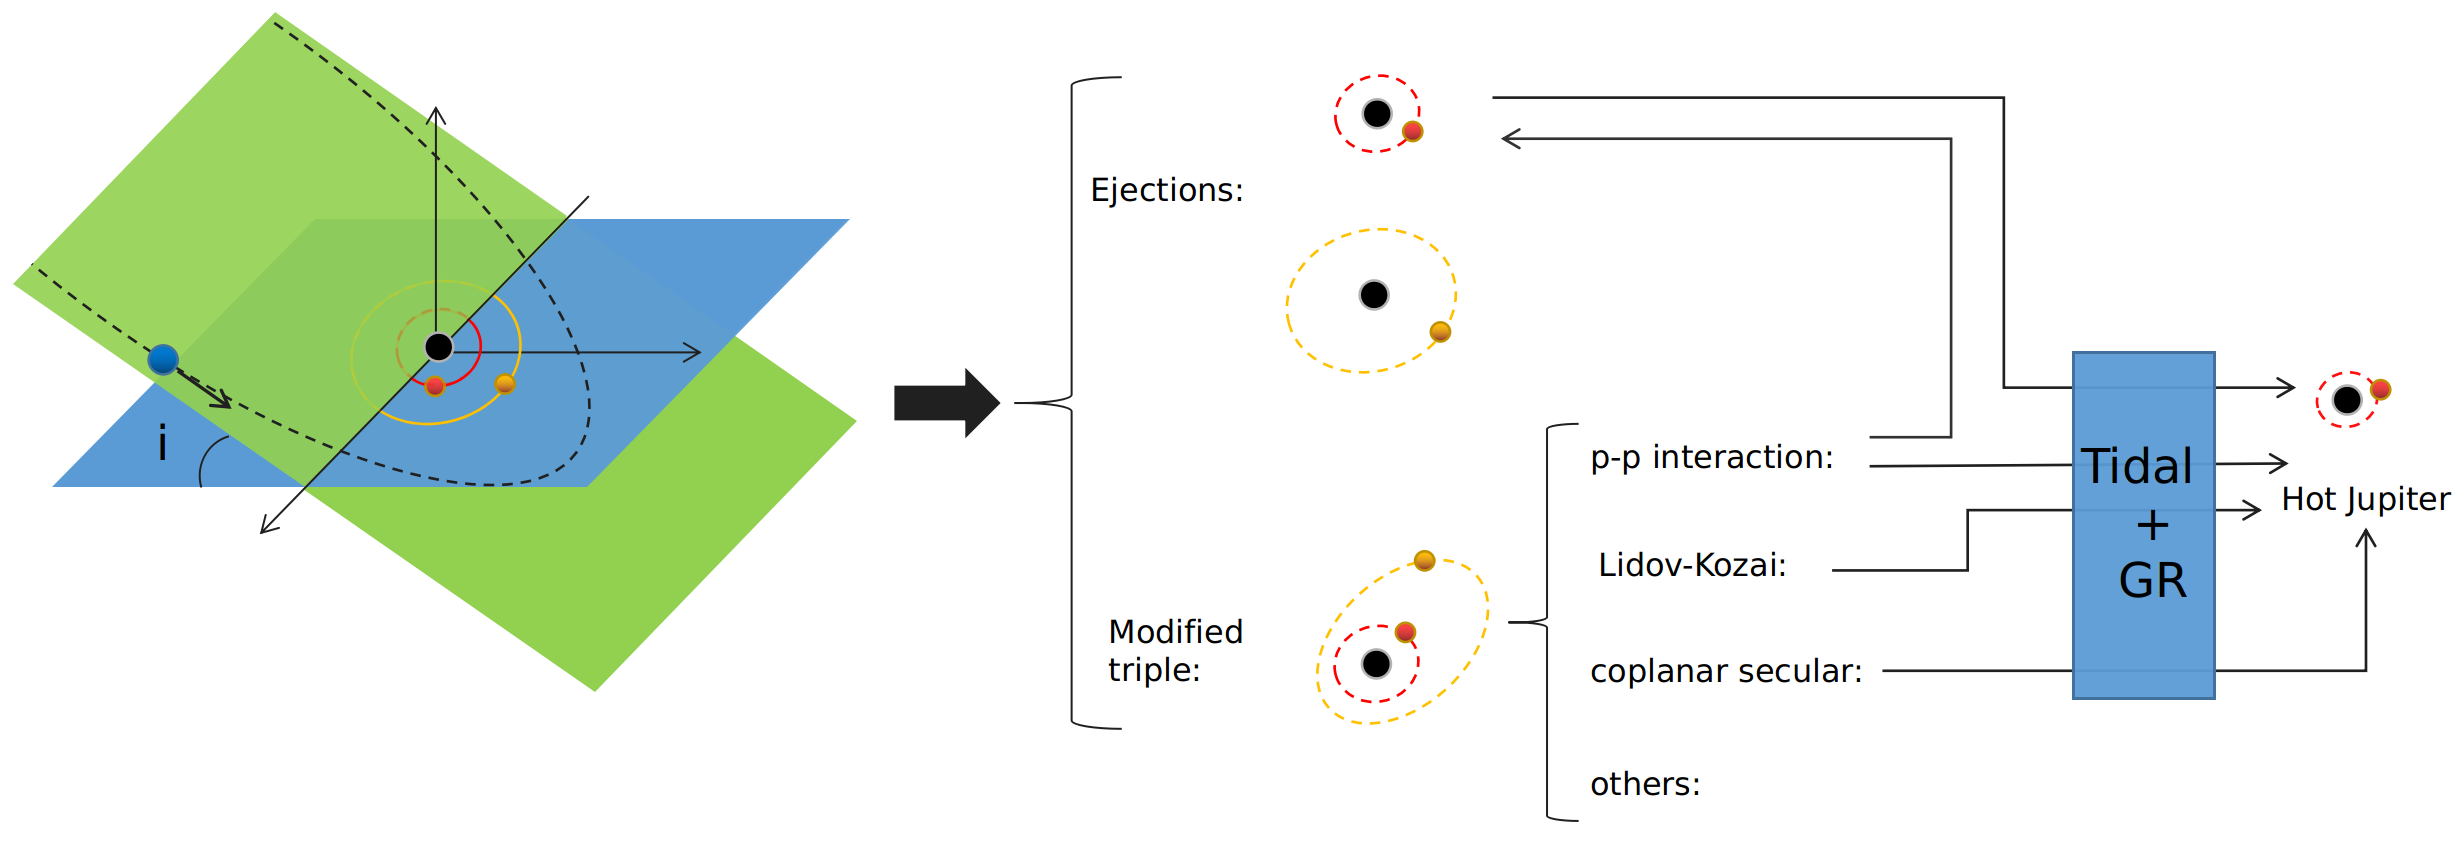
\includegraphics[width=\textwidth]{schematics}
	\caption{Schematic illustration of the flyby and long time interactions. After the flyby, the planet system will be modified. If the structure of the planet system keep intact, the modified triple may form configuration in planet-planet interaction regime, Lidov-Kozai regime and coplanar secular regime. In those regime, the eccentricity of the Jupiter can be excited to high value, which make the hot Jupiter possible due to the tidal circularization.}
	\label{fig:schematics}
\end{figure*}


\begin{figure*}
	\includegraphics[width=\textwidth]{regimes-after-flyby-ratio2}
	\caption{This plot shows the regime of the outcomes after the flyby. The x-axis is the pericenter of the Saturn / apocenter of the Jupiter, while the y-axis is the inclination between the two planet orbits. The initial semi-major axis(SMA) of the Jupiter $a_{j,0}$= 5.2 AU, and the initial SMA of the Saturn $a_{s,0}/a_{j,0}=2$. }
	\label{fig:schematics}
\end{figure*}

\begin{figure*}
	\includegraphics[width=\textwidth]{regimes-fraction-after-flyby-ratio2}
	\caption{In each subplot, the {\color{green}left side} of the green line shows the fraction of the outcome after the flyby. \textit{J-ejctn}: Jupiter get ejected but Saturn remains; \textit{S-ejctn}: Saturn get ejected but Jupiter remains; \textit{B-ejctn}: Both planets get ejected; \textit{remain}: Both planets remain. On the {\color{green}right side} of the green line, for \textit{remain} systems, here shows the fraction in different regimes(LK:Lidov-Kozai; p-p:planet-planet interaction; stable:stable without eccentricity excitation; unstable:unstable system.) }
	\label{fig:schematics}
\end{figure*}

\begin{figure*}
	\includegraphics[width=\textwidth]{tidal-final-a}
	\caption{The distribution of the final SMA of the Jupiter at 1 Gy. The simulations a bit slow after we add the tidal dissipation. The simulation costs 99\% of the time in the final stage where $a_j$ is tiny(thus much short time step). Here the questions is :in each regime, what's the fraction of the HJ after 1Gy integration. Then, we can estimate the fraction of the HJ from different channels(which is created by flyby). However, the current results cannot give an accurate estimation on these fraction due to the small HJ data set(need to run longer). }
	\label{fig:schematics}
\end{figure*}


\begin{figure*}
	\includegraphics[width=\textwidth]{regimes-after-flyby-ratio4}
	\caption{\textbf{The initial planet SMA ratio affects the fraction of the system in different regimes after the flyby. Thus we change the ratio from 2 to 4}. This plot shows the regime of the outcomes after the flyby. The x-axis is the pericenter of the Saturn / apocenter of the Jupiter, while the y-axis is the inclination between the two planet orbits. The initial semi-major axis(SMA) of the Jupiter $a_{j,0}$= 5.2 AU, and the initial SMA of the Saturn $a_{s,0}/a_{j,0}=${\color{red} 4}. }
	\label{fig:schematics}
\end{figure*}

\begin{figure*}
	\includegraphics[width=\textwidth]{regimes-fraction-after-flyby-ratio4}
	\caption{The same plot but with $a_{s,0}/a_{j,0}=${\color{red} 4}.}
	\label{fig:schematics}
\end{figure*}


\begin{figure*}
	\includegraphics[width=\textwidth]{regimes-after-flyby-ratio8}
	\caption{The same plot but with $a_{s,0}/a_{j,0}=${\color{red} 8}.}
	\label{fig:schematics}
\end{figure*}

\begin{figure*}
	\includegraphics[width=\textwidth]{regimes-fraction-after-flyby-ratio8}
	\caption{The same plot but with $a_{s,0}/a_{j,0}=${\color{red} 8}.}
	\label{fig:schematics}
\end{figure*}



\begin{figure*}
	\includegraphics[width=\textwidth]{3d-0deg}
	\caption{The 3D plot, with {\color{red}incident angle i = 0 deg}.$a_{j,0}$=5.2 au and $a_{s,0}/a_{j,0}=2$.}
	\label{fig:schematics}
\end{figure*}

\begin{figure*}
	\includegraphics[width=\textwidth]{3d-30deg}
	\caption{The 3D plot, with {\color{red}incident angle i = 30 deg}.$a_{j,0}$=5.2 au and $a_{s,0}/a_{j,0}=2$.}
	\label{fig:schematics}
\end{figure*}


\begin{figure*}
	\includegraphics[width=\textwidth]{3d-60deg}
	\caption{The 3D plot, with {\color{red}incident angle i = 60 deg}.$a_{j,0}$=5.2 au and $a_{s,0}/a_{j,0}=2$.}
	\label{fig:schematics}
\end{figure*}

\begin{figure*}
	\includegraphics[width=\textwidth]{3d-90deg}
	\caption{The 3D plot, with {\color{red}incident angle i = 90 deg}.$a_{j,0}$=5.2 au and $a_{s,0}/a_{j,0}=2$.}
	\label{fig:schematics}
\end{figure*}
% The MNRAS class isn't designed to include a table of contents, but for this document one is useful.
% I therefore have to do some kludging to make it work without masses of blank space.


% Please add the following required packages to your document preamble:
% \usepackage{multirow}



\begingroup
\let\clearpage\relax
\tableofcontents
\endgroup
\newpage

\section{Introduction}





\section*{Acknowledgements}


%%%%%%%%%%%%%%%%%%%%%%%%%%%%%%%%%%%%%%%%%%%%%%%%%%

%%%%%%%%%%%%%%%%%%%% REFERENCES %%%%%%%%%%%%%%%%%%

% The best way to enter references is to use BibTeX:

%\bibliographystyle{mnras}
%\bibliography{example} % if your bibtex file is called example.bib


% Alternatively you could enter them by hand, like this:
\begin{thebibliography}{99}

\end{thebibliography}




% Don't change these lines
\bsp	% typesetting comment
\label{lastpage}
\end{document}

% End of mnras_guide.tex